\chapter{Aufgaben Erweiterung}
Patrick Niepel \& Marcel Hagmann \& Carl Philipp Knoblauch

\section{Einleitung}
Unsere erste Aufgabe war die Erweiterung der Stundenlpan App um ein Aufgaben Feature. Mit dem Aufgaben Feature kann der Nutzer seine Aufgaben aus Vorlesungen in die App eintragen. Diese werden auch in die Kalender synchronisiert.

\newpage
\section{Planung}

Die Planung unserer ersten Aufgabe began schon bevor wir diese bekommen haben. In der ersten Vorlesung sollten wir uns in Gruppen zusammen finden und überlegen, welche Aufgaben wir machen wollen. Dafür haben wir eine Aufgaben Erweiterung vorgeschlagen und die Funktionen auch schon geplant.

\subsection{Mockup}

Bevor wir uns an die eigentliche Programmierung gemacht haben, erstellten wir ein Mockup zu unserer Idee. Dieses Mockup konnten wir auch sehr gut umsetzen. Die Farben haben sich allerdings, wegen einer späteren Aufgabe für unsere Gruppe, wieder geändert. (Universal App Design)


\begin{figure}[ht]
	\centering
  \frame{ 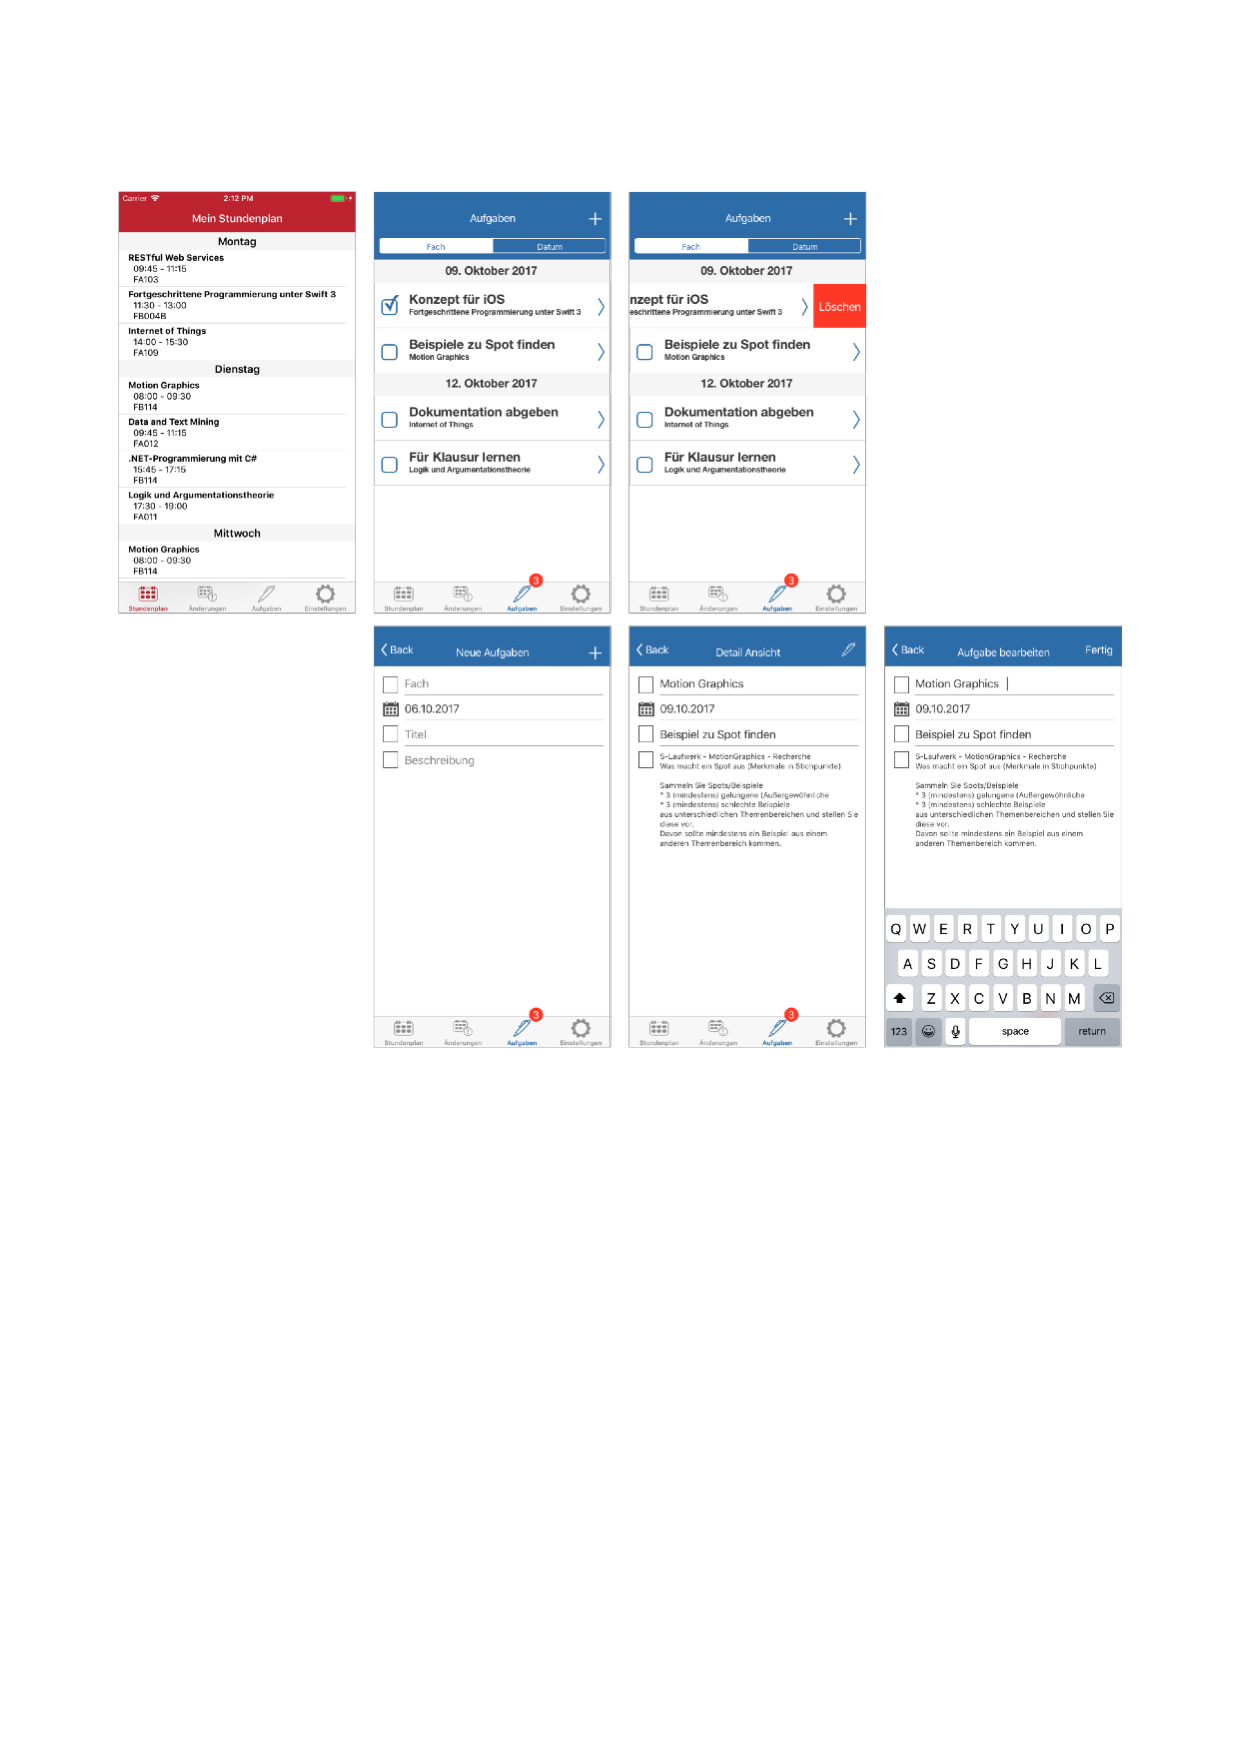
\includegraphics[width=0.9\textwidth]{Mockup_ios_aufgaben} }
	\caption{Mockup unserer Aufgaben Erweiterung}
	\label{fig1}
\end{figure}

\newpage
\section{Umsetzung}
